% Method verified against the current AV + Whisper + Feature + LTX clip-Event code.
% Source map, equations, and remaining author decisions: review/方法重写与实现核对_20261108.md.
\section{Method}
\label{sec:method}

\begin{figure*}[t]
\centering
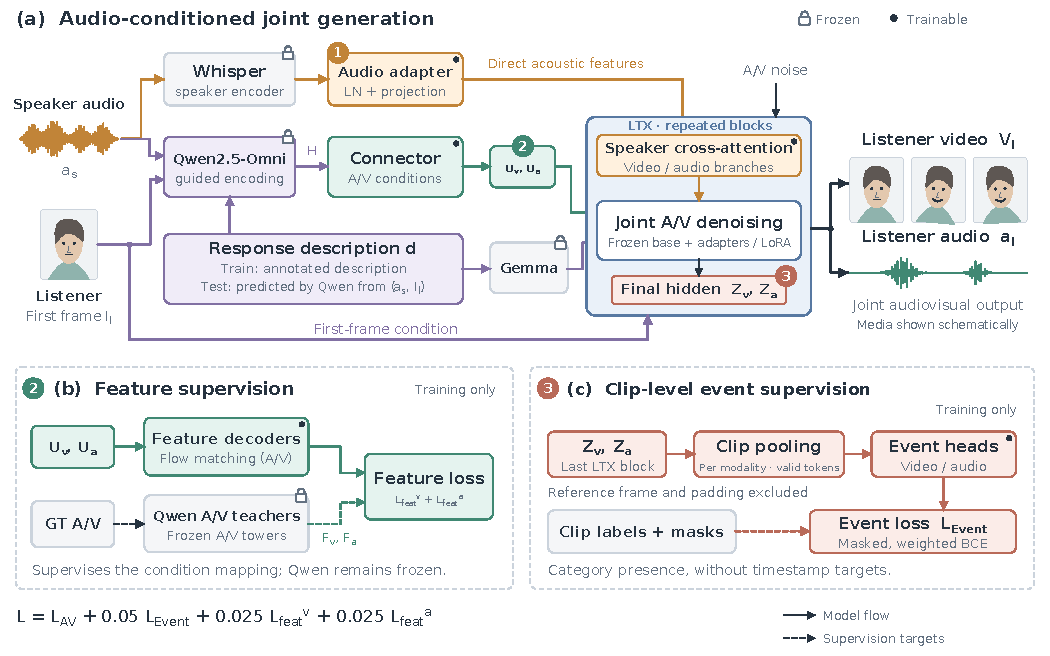
\includegraphics[width=\textwidth]{F3_method.pdf}
\caption{\figdraft{F3: Generation framework and training supervision} A connector maps guided Qwen representations to video and audio conditions, which are appended to Gemma text conditions. An independent Whisper path supplies speaker-audio features to both LTX streams. Feature supervision trains the condition mapping with frozen target-media features; clip-level Event supervision reads the final LTX block. Training uses annotated descriptions, whereas inference predicts and re-encodes descriptions from the permitted inputs. Both auxiliary objectives are used only during training. Portraits and waveforms are schematic.}
\label{fig:method}
\end{figure*}

\subsection{Task Definition and Overview}
\label{sec:conditioning}
% Included inside Method 3.1 by 05_method.tex; this file adds no numbered heading.
\label{sec:task}
\paragraph{Task definition.}
% Paragraph role P01: 任务——当前语音与首帧到同时间段的倾听视听反馈。
Given the current speaker audio $a_s$ and the listener's first frame $I_l$,
we generate listener video $V_l$ and audio $a_l$ over the corresponding
interval. We focus on feedback while the speaker holds the conversational
floor, including facial reactions, head movements, and brief vocal
acknowledgments. Quiet listening is also valid. The input does not uniquely
determine the listener's reaction or its timing, and an observed response
is one possible realization. At inference, the model receives no dialogue
history, speaker video, target listener audio, or reference reaction labels.
\cnnote{统计待补}{应用面向一两句当前话语；训练与测试的实际片段长度及句数分布仍需报告，不能把应用设定直接写成已统计确认的数据分布。}

% Paragraph role P02: 监督接口——先说明方法使用哪些数据，构建细节放第4章。
Training uses paired listener audiovisual media, an ordered reaction
description $d^*$, and clip-level behavior labels with validity masks.
These descriptions and labels are derived from the target media during
data construction (\cref{sec:data}); they are supervision, not additional
inputs required from the user.


\paragraph{Generation conditions.}
% Paragraph role P01: 总览——理解条件、直接声学条件与联合生成器的分工。
Our framework combines a description-conditioned representation of the
intended response with direct acoustic information from the speaker
(\cref{fig:method}). A frozen Qwen2.5-Omni model~\cite{qwen25omni} encodes
the speaker audio, listener image, and a reaction description $d$ into
multilayer hidden states $H$. A trainable connector $C_\theta$ produces
separate video and audio conditions, while Gemma~\cite{gemma_pending}
encodes the same description. For modality $m\in\{v,a\}$, we write
\begin{equation}
 (U_v,U_a)=C_\theta(H),\qquad c_m=[G_m(d);U_m],
\label{eq:conditions}
\end{equation}
where $G_m(d)$ is the processed Gemma context for that stream and brackets
denote token concatenation. The joint LTX generator~\cite{ltx_pending}
uses $c_v$, $c_a$, the reference frame, and the speaker-audio features
introduced below to generate both listener modalities.

% Paragraph role P02: Connector——层感知记忆与坐标查询将Qwen表征映射到两路条件。
The connector normalizes and projects each selected Qwen layer into a
shared memory, adding learned layer embeddings before concatenation.
Video and audio queries are initialized from feature-grid coordinates
and modality embeddings. Each fusion block applies cross-attention to
the Qwen memory, self-attention across the combined query sequence, and
a feed-forward network. Separate output projections produce $U_v$ and
$U_a$ in the dimensions required by the two LTX context streams. This
provides a trainable interface between frozen understanding and generation
models. The final projection topology follows Bernini~\cite{bernini_pending};
the coordinate-query fusion defines how information is gathered from the
selected Qwen layers.

% Paragraph role P03: 描述来源——训练用标注，推理预测并重新编码，描述是内部条件。
During training, $d=d^*$ is the annotated description of the target
response. It is appended as assistant guidance after Qwen's multimodal
input prefix, and the resulting sequence supplies $H$. During inference,
Qwen first predicts $\hat d$ from $a_s$, $I_l$, and the task instruction;
we then re-encode this description to obtain $H$ and $G_m(\hat d)$.
The description is thus an internal condition. Direct acoustic
conditioning supplements this representation, while Feature and Event
supervision respectively target the condition mapping and generated
feedback behavior.

\subsection{Direct Speaker-Audio Conditioning}
\label{sec:direct-audio}
% Paragraph role P04: Whisper动机与设计——保留直接声学信息，补充描述与高层条件。
A reaction description summarizes intended behavior, but does not
explicitly preserve every local acoustic cue in the speaker's utterance.
We therefore provide a separate path from speaker audio to the generator.
A frozen Whisper-large-v3 encoder~\cite{whisper} extracts a temporal
feature sequence; a trainable LayerNorm and linear adapter map it to
speaker context $S$. Independent cross-attention branches inject $S$
into the video and audio streams of every LTX block:
\begin{equation}
 h_{b,m}\leftarrow h_{b,m}
 +\operatorname{CA}_{b,m}(h_{b,m},S),\quad m\in\{v,a\},
\label{eq:speaker-attention}
\end{equation}
where $b$ indexes a block. Generation features provide queries, and
speaker features provide keys and values. These branches supplement
the existing attention to $c_m$ in \cref{eq:conditions}.

% Paragraph role P05: 时间与初始化——共同时间坐标、保留静音、无额外Whisper损失。
Speaker keys and generation queries use temporal rotary positions
defined on a common time origin in seconds. Padding is masked, and
leading and internal speaker silence are retained. The additional output
projections are initialized to zero, preserving the original path at
initialization. The adapter and attention branches learn through the
generation and Event objectives; there is no separate Whisper loss.
The model can attend to the supplied audio segment as a whole and does
not impose streaming causality.

\subsection{Target Audiovisual Feature Supervision}
\label{sec:feature}
% Paragraph role P06: Feature动机——让实际送入生成器的条件携带目标媒体信息。
The connector must transform general multimodal representations into
conditions useful for listener generation. To supervise this mapping,
we extract target features $F_v$ and $F_a$ from real listener video and
processed audio using frozen Qwen visual and audio encoders. The queries
that produce $U_m$ are organized to correspond to these teacher-feature
positions. An auxiliary decoder $D_{\phi_m}$ for each modality learns
to recover target features conditioned on $U_m$, following the
AdaLN-modulated feature-decoder design of Bernini~\cite{bernini_pending}.

% Paragraph role P07: Feature公式——独立噪声下的特征流匹配，保留有效位置与安静音频。
For each valid feature position, we sample Gaussian noise $\epsilon$
and a noise level $\sigma\sim\mathcal U(0,1)$, forming
$x_{\sigma,m}=(1-\sigma)F_m+\sigma\epsilon$. The decoder predicts
the flow velocity toward noise, with objective
\begin{equation}
 \mathcal L_{\mathrm{Feature}}^m =
 \mathbb E_{\sigma,\epsilon}\!\left[
 \big\|D_{\phi_m}(x_{\sigma,m},\sigma,U_m)
       -(\epsilon-F_m)\big\|_{\Omega_m}^{2}\right].
\label{eq:feature}
\end{equation}
Here the squared norm averages over channels and positions in
$\Omega_m$, where both the teacher feature and condition are valid;
the training loss is also averaged over samples. Silence is a valid
audio target and is not excluded solely because no vocalization occurs.

% Paragraph role P08: Feature梯度——监督Connector，冻结Qwen，推理无需教师或解码器。
Because the decoders consume the same $U_m$ used by LTX, their gradients
encourage the connector to retain information relevant to the target
listener media. This is a conditional feature-reconstruction objective,
not a direct regression between Qwen hidden states and teacher features.
The connector and auxiliary decoders are trainable; the Qwen backbone
and teacher encoders remain frozen. Neither target features nor auxiliary
decoding is required at inference.

\subsection{Clip-Level Event Supervision}
\label{sec:event}
% Paragraph role P09: Event动机与读出——从生成表征而非条件U监督反馈类别存在。
The continuous audiovisual objective does not explicitly specify which
feedback categories should occur. We therefore attach visual and audio
event heads to the generation representations of LTX. In each training
forward pass, we read hidden states $Z_v$ and $Z_a$ from the final
Transformer block, before output normalization and projection. Video
states are averaged spatially within each valid time position and then
temporally; audio states are averaged over their valid temporal positions.
Pooling excludes reference-frame tokens, padding, and positions outside
the actual generation support. Separate LayerNorm--MLP heads map the
pooled representations to clip-level category logits.

% Paragraph role P10: Event标签与公式——区分正例、弱负例和未知，按有效样本归一化。
The targets are derived from reaction descriptions with the evidence
checks described in \cref{sec:annotation}. For sample $i$ and class $c$,
$y_{ic}\in\{0,1\}$ denotes category presence, $M_{ic}$ indicates a valid
target, and $w_{ic}$ controls its weight. Accepted positives have weight
1; unmentioned categories receive weak-negative weight 0.1 only when
the description passes the completeness checks. Uncertain or conflicting
entries are masked. We use class-weighted binary cross-entropy:
\begin{equation}
 \mathcal L_{\mathrm{Event}}=
 \frac{1}{|\mathcal C_{\mathrm{eff}}|}
 \sum_{c\in\mathcal C_{\mathrm{eff}}}
 \frac{\sum_i M_{ic}w_{ic}\,
       \mathrm{BCE}_{\alpha_c}(s_{ic},y_{ic})}
      {\sum_i M_{ic}},
\label{eq:event}
\end{equation}
where $s_{ic}$ is a logit, $\alpha_c$ is a positive-class weight derived
from training statistics, and $\mathcal C_{\mathrm{eff}}$ contains enabled
classes with valid targets in the training batch. Normalization uses the
number of valid samples rather than their weight sum, preserving the
reduced influence of weak negatives.

% Paragraph role P11: Event作用边界——整段存在性适配可变时序，但不保证所有生成行为正确。
This objective supervises whether a category occurs within the clip,
without imposing event start or end times. It accommodates variation in
feedback timing while the audiovisual objective continues to supervise
the paired media. Event heads read hidden states at the sampled
flow noise level, so training requires no additional full video sampling
or decoding. Their gradients pass through the trainable LTX branches to
the connector. The heads are not executed at inference; their predictions
are not used to score generated videos. The training behavior vocabulary
and the evaluation categories are defined separately.

\subsection{Training and Inference}
\label{sec:training}
\paragraph{Joint objective.}
% Paragraph role P12: AV目标——双路潜空间流匹配，固定参考首帧并屏蔽无效支持。
The native audiovisual objective trains LTX to jointly predict video and
audio flow velocities. Let $x_0^m$ be a target latent encoded by the frozen
modality VAE. At a sampled noise level $\tau$, we form
$x_\tau^m=(1-\tau)x_0^m+\tau\epsilon_m$ at generated positions.
The reference-frame latent stays clean and fixed. Writing the joint
generator's output for stream $m$ as $v_\Theta^m$, the loss is
\begin{equation}
 \mathcal L_{\mathrm{AV}}=
 \mathbb E\!\left[
 \sum_m
 \big\|v_\Theta^m(x_\tau^v,x_\tau^a,\tau;\mathcal K)
       -(\epsilon_m-x_0^m)\big\|_{\Lambda_m}^{2}\right],
\label{eq:av}
\end{equation}
where $\mathcal K$ collects the reference-frame, Qwen/Gemma, and Whisper
conditions. $\Lambda_m$ is the valid generation mask, excluding fixed
reference positions and padding; the norm is a mean over valid positions
and channels, and the expectation includes training samples and noise.

% Paragraph role P13: 总目标——Whisper是条件路径，Feature与Event是辅助监督。
The complete model uses
\begin{equation}
\begin{split}
 \mathcal L ={}& \mathcal L_{\mathrm{AV}}
       +0.05\mathcal L_{\mathrm{Event}}\\
       &+0.025\mathcal L_{\mathrm{Feature}}^v
        +0.025\mathcal L_{\mathrm{Feature}}^a.
\end{split}
\label{eq:total}
\end{equation}
We train the connector, Whisper adapter and attention branches, auxiliary
feature decoders, event heads, and LoRA adapters in LTX's native video and
audio text cross-attention. The Qwen, Gemma, Whisper, and VAE encoders,
target-feature teachers, and pretrained LTX backbone weights remain
frozen. Feature supervision acts on the condition mapping; Event
supervision reaches that mapping through the generation network.

\paragraph{Inference.}
% Paragraph role P14: 推理——预测描述、构建条件、联合采样，保持训练外目标不可见。
Given $a_s$ and $I_l$, Qwen predicts $\hat d$ and re-encodes it to construct
the guided hidden states; Gemma encodes the same description. The
connector produces $U_v$ and $U_a$, while Whisper supplies direct speaker
features. LTX jointly samples video and audio latents from noise, keeping
the reference-frame latent fixed, and decodes the listener response.
Both classifier-free guidance branches retain the Qwen and Whisper
conditions; the negative branch uses empty Gemma text. No target listener
media, annotated descriptions, teacher features, or event labels are
accessed. Model versions and sampling settings are specified in
\cref{sec:setup}.
